\section{PMT Characterization}
\label{PMT_char_app}

The detection region of the \CENTREX\ experiment uses a set of approx.\ five
\gls{PMT} detectors (Hamamatsu R375). While the datasheet indicates the
approximate relationship between the incident light and the output signal, in
practice there is a significant variation between different units of the same
model. In this section, we will present the testing apparatus we have used to
calibrate the \gls{PMT} output at a given light power level, the calibration
procedure, and the test results.

\subsection{Measurement apparatus}

Fig.~\ref{PMT_testing_setup} shows an outside and inside view of the apparatus.
The \gls{PMT} under test is contained within an aluminum tube (3" outer
diameter, 1/4" wall thickness, 12" long, McMaster p.n.\ 9056K21) together with
the light source (UV \gls{LED}, Quelighting Corp p.n.\ QLUV07N2DM, mounted on a small
custom PCB with a BNC connector for the constant current supply) and electronic
connections for the \gls{PMT}: a \gls{PMT} socket (Hamamatsu E1435-02) soldered
to a BNC connector (Molex 0731315003) for the signal output, and a SHV connector
(TE 51494-2) for the negative cathode high voltage supply.

\begin{figure}
  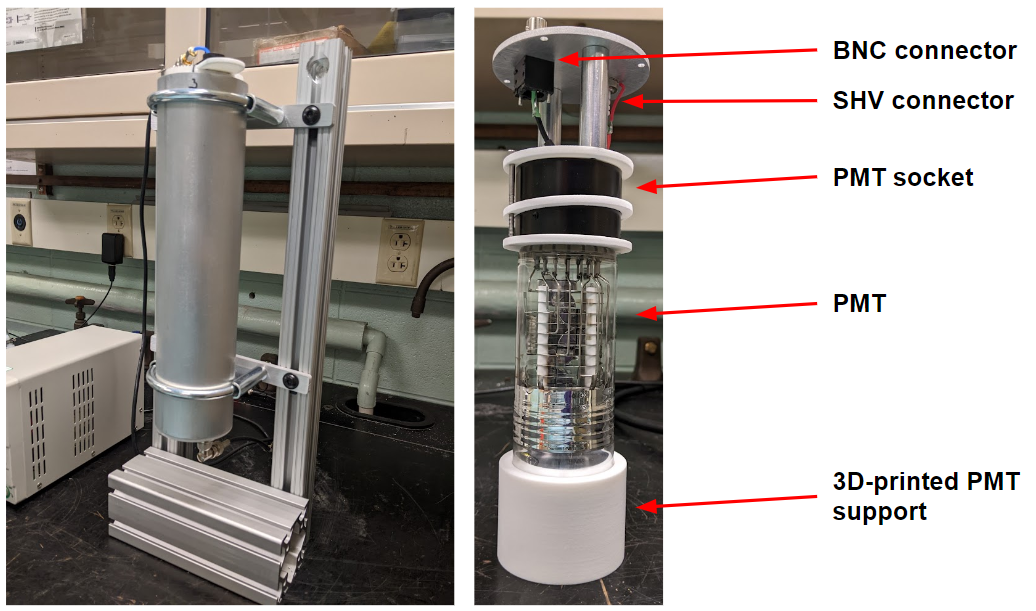
\includegraphics[width=\textwidth]{figs/todo/PMT.png}
    \caption[\gls{PMT} characterization apparatus.]{\gls{PMT} characterization
    apparatus. \part{Left} Contained inside an aluminum tube. \part{Right} Inner
    assembly, including the \gls{PMT} under test, but excluding the optics
    (\gls{LED} light source, filters, diffusor plates).}
    \label{PMT_testing_setup}
\end{figure}

The aluminum tube is closed on both ends with 1/8" thick aluminum plates. The
bottom end plate contains a cutout for the BNC connector to supply the current
for the \gls{LED} light source. Stacked on top of the bottom plates is an O-ring (Buna-N,
dash number 405, McMaster p.n.\ 9452K501), approx.\ 2" long segment of an UHMW
plastic tube (McMaster p.n., 8705K23), another O-ring, and a custom aluminum
plate (1/8" thick) with cutouts to attach a flange-to-SM1 adapter (Thorlabs p.n.
SM1F1), from which a short lens tube can be suspended, holding the optics. Refer
to Fig.~\ref{bottom_assy} for a rendered view. The entire assembly is clamped to
a simple 80/20 frame (Fig.~\ref{PMT_testing_setup}, left) that is kept in the
same position throughout the testing. The setup does not contain magnetic
shielding.

\begin{figure}
   \centering
  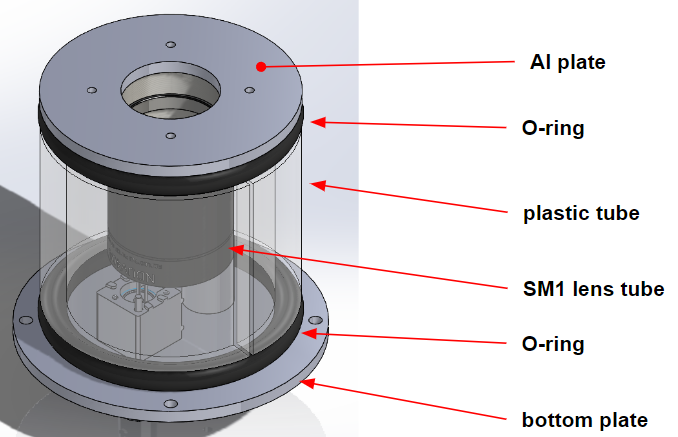
\includegraphics[width=.6\textwidth]{figs/todo/bottom_assy.png}
    \caption[Bottom part of \gls{PMT} testing apparatus.]{Bottom part of the
    test apparatus assembly, containing the light source (\gls{LED}, not shown)
    and filtering optics (contained within the lens tube).}
  \label{bottom_assy}
\end{figure}

\subsection{Calibration procedure}

Before the setup is used for testing individual \glspl{PMT}, we calibrate the
amount of light emitted by the \gls{LED} as a function of transverse position. To do
so, we replace the top part of the assembly that normally contains the \gls{PMT}
with an assembly that holds a photodiode in a sliding mount
(Fig.~\ref{sliding_mount}). The top plate consists of two parts (3D printed from
nylon 12), such that the photodiode (silicon, 200--1100~nm, Thorlabs SM05PD2A),
located at the end of the long lens tube, can be scanned in the radial and
azimuthal directions. Inside the shorter lower lens tube we mount three 120 grit UVFS
diffuser plates (Thorlabs DGUV10-120) as well as a colored glass filter
(245--400~nm, Thorlabs FGUV11-UV). The three diffuser plates are stacked with
approx.\ 1/2" space between them to create an approximately Gaussian light
source (Fig.~\ref{diffusors}, right), which is preferable over the rectangular
\gls{LED} shape (Fig.~\ref{diffusors}, left) since it covers a broader area.

\begin{figure}
  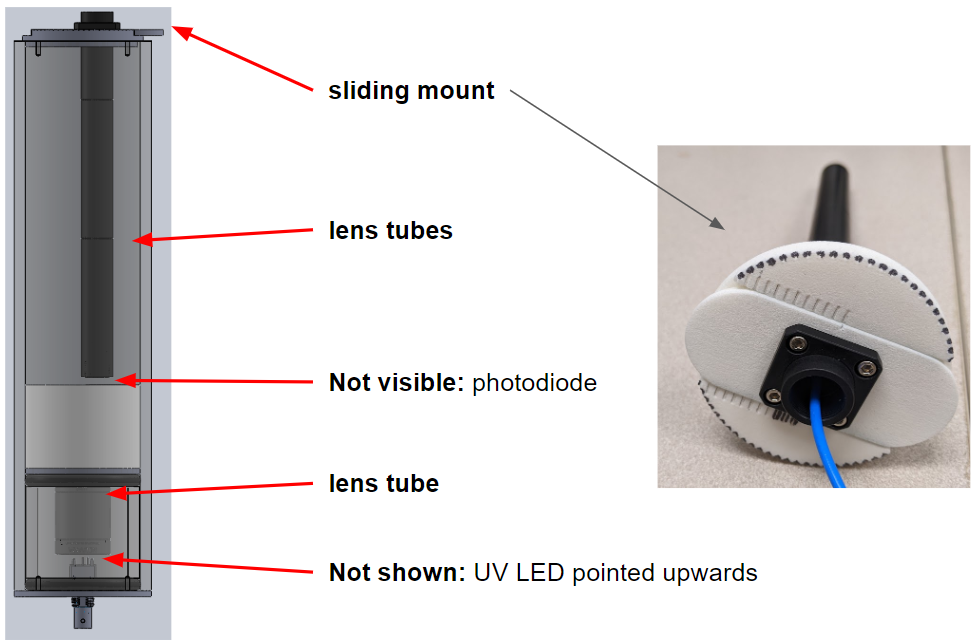
\includegraphics[width=\textwidth]{figs/todo/sliding_mount.png}
   \caption{Setup for light power calibration inside the \gls{PMT} testing setup.}
  \label{sliding_mount}
\end{figure}

\begin{figure}
  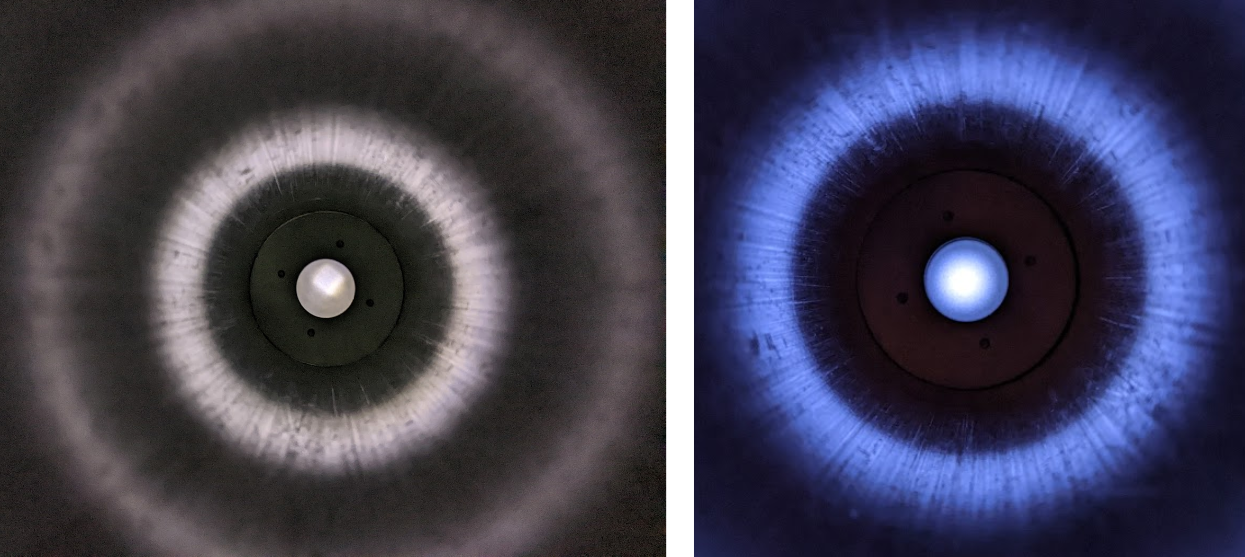
\includegraphics[width=\textwidth]{figs/todo/diffusors.png}
    \caption[Diffuser plates to increase \gls{LED} uniformity.]{The view down
    the outer aluminum tube towards the light source.  \part{Left} When the
    three diffuser plates are stacked on top of each other, the square shape of
    the \gls{LED} can be seen. \part{Right} When the three diffuser plates are
    stacked with approx.\ 1/2" space between them, the source appears
    approximately Gaussian.}
  \label{diffusors}
\end{figure}

The photodiode signal is amplified by a 1~kHz bandwidth transimpedance amplifier
with 10~MV/A gain (Thorlabs AMP110) and read out on an oscilloscope. From their
respective datasheets, we obtain the spectrum of the \gls{LED} and the bandpass
filter. By integrating the response of the photodiode over that spectrum, we
find that the photodiode gain is approx.\ 32.1~mA/W. Thus we can estimate the
light intensity as a function of transverse position as shown in
Fig.~\ref{spatial_distn} together with Gaussian fits. By integrating the fits
over a 46~mm diameter circle (the diameter of the \gls{PMT} photocathode), we
find that approx.\ 45\%\ of the emitted light is within this diameter. The
photodiode is significantly smaller (0.8~mm$^2$) than the \gls{PMT} and receives
1593$\times$ less light.

The amount of light observed and reported in Fig.~\ref{spatial_distn} would
overwhelm the \gls{PMT}. At an approximate gain of $10^5$ and cathode
sensitivity 49.3~mA/W, the light power needs to be limit to below 20~nW to keep
the anode current below the maximum value of 0.1~mA. At a \gls{LED} current of 25~mA
as used in the above tests, the photodiode receives approx.\ 100~nW of light.
Since the \gls{PMT} covers approx.\ 2000$\times$ the area, the light needs to be
attenuated by a factor of 10,000 (ND 4.0). With such attenuation, the photodiode
would receive a mere 0.01~nW of light, corresponding to a 0.4~pA photodiode
current, which is well below the 0.3~nA dark current. We thus insert a
reflective ND filter (Thorlabs NDUV40A) when the photodiode calibration is
completed to adapt the setup for \gls{PMT} calibration.

The \gls{PMT} anode current is converted to a voltage using a 50~$\Omega$
termination, amplified by a variable-gain precision voltage amplifier (Stanford
Research Systems SR560) and read out by an oscilloscope.

\begin{figure}
  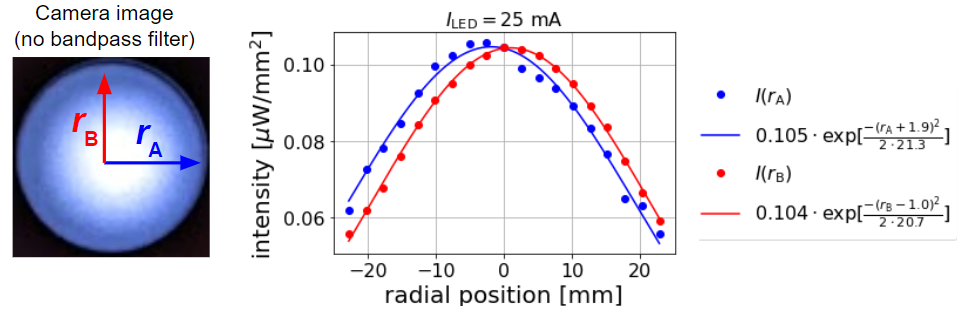
\includegraphics[width=\textwidth]{figs/todo/spatial_distn.png}
   \caption{Spatial light distribution.}
  \label{spatial_distn}
\end{figure}

\subsection{Results}

We define the \gls{PMT} gain as a function of the anode current $I_\text{anode}$
as follows:
%
\begin{align}
   \label{PMT_gain}
   \text{PMT gain}=\text{ND}\cdot\frac{I_\text{anode}}{\int\rho_\text{\gls{LED}}\cdot
   R_\text{PMT}\;\d\lambda}/P_\text{PD}(I_\text{\gls{LED}}),
\end{align}
%
where ND is the attenuation of the ND filter (nominally 10,000). The integral in
the denominator is the integrated \gls{PMT} cathode sensitivity of 49.3~mA/W,
and $P_\text{PD}(I_\text{\gls{LED}})$ is the power incident on the photodiode at a
given \gls{LED} current $I_\text{\gls{LED}}$, multiplied by the area factor 1593. See
Fig.~\ref{SB4715} for gain curves measured at a range of different cathode
voltages and incident light levels. The left plot shows the \gls{PMT} gain as
per eqn~\ref{PMT_gain} as a function of cathode voltage, while the right plot
directly shows the anode current as a function of light input. We see that the
\gls{PMT} output becomes nonlinear as the light power increases and the detector
exhibits saturation effects.

\begin{figure}
  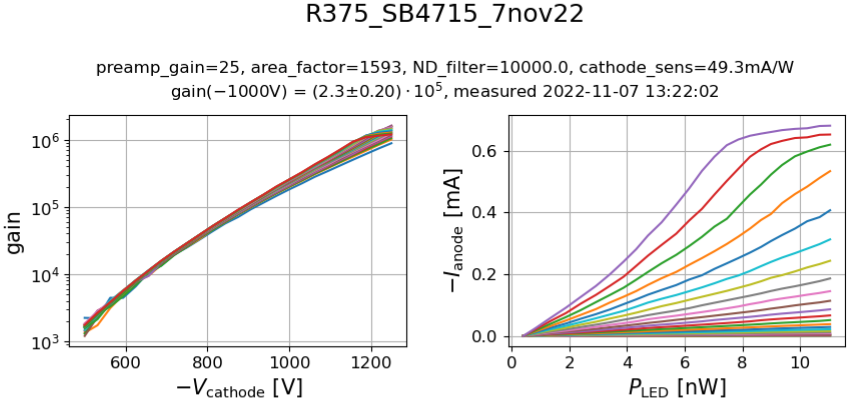
\includegraphics[width=\textwidth]{figs/todo/SB4715.png}
    \caption[Example measurement results for one \gls{PMT}.]{Example measurement
    results for one \gls{PMT}. The two plots show the same data (2D scan of
    \gls{PMT} output vs cathode voltage and \gls{LED} power), just transposed
    and plotted in different units. \part{Left} Gain curves as a function of
    cathode voltage, for \gls{LED} power ranging from 0.4 to 10.7 nW.
    \part{Right} Anode current as a function of \gls{LED} power, with cathode
    voltage ranging from $-500$~V (least negative current) to $-1250$~V (most
    negative current).}
  \label{SB4715}
\end{figure}

In the linear regime with respect to the incident light power levels, the anode
current follows a power law relationship with the cathode voltage:
%
\begin{equation}
   \label{anode_current_vs_voltage}
   \begin{aligned}
      I_\text{anode}&=a\cdot
      P_\text{light}\left(-V_\text{cathode}/100~\text{V}\right)^k\\
      -V_\text{cathode}&=100~\text{V}\left[I_\text{anode}/\left(a\cdot
      P_\text{light}\right)\right]^{1/k}
   \end{aligned}
\end{equation}
%
We fit the measured data to this equation to extract the fit parameters $a$ and
$k$. These are reported in Table~\ref{PMT_test_results}. The expression can also
be rearranged to give the \gls{PMT} gain at a given cathode voltage:
%
\begin{equation}
   \label{PMT_gain_eqn}
   \text{gain}=
   \frac
   {a\cdot\left(-V_\text{cathode}/100~\text{V}\right)^k}
   {\int\rho_\text{\gls{LED}}\cdot R_\text{PMT}\;\d\lambda},
\end{equation}
%
where again the denominator is the integrated \gls{PMT} cathode sensitivity of
49.3~mA/W. The gain can also be calculated from the values reported by the
manufacturer in the test sheets supplied with the photomultiplier; these values
are also reported in Table~\ref{PMT_test_results}.

\begin{figure}
   \centering
  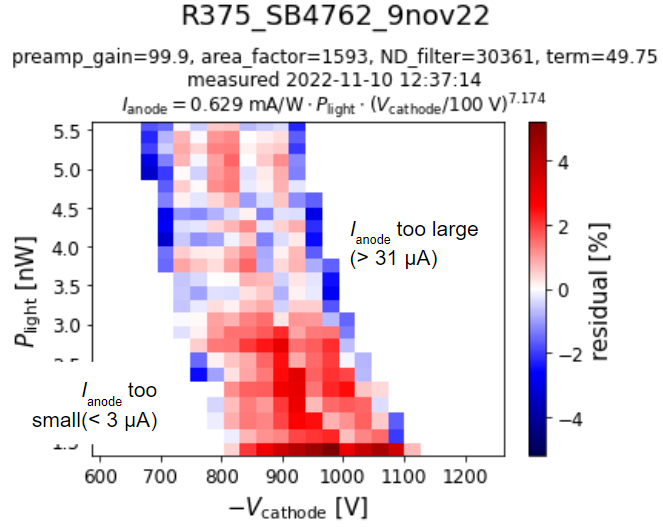
\includegraphics[width=.6\textwidth]{figs/todo/PMT_res.png}
    \caption[Fit residuals for \gls{PMT} data.]{Fit residuals when fitting
    measured data to eqn~\ref{anode_current_vs_voltage} for a particular
    \gls{PMT} unit. We exclude data points where the anode current is too small
    (data too noisy) or too large (indicating detector nonlinearity as it
    saturates).}
  \label{PMT_res}
\end{figure}

\begin{table*}
  %\small
  \makebox[\textwidth][c]{%
    \begin{tabu} to \textwidth {cccccccc}
      \toprule
       Serial & $a$    & $k$ & $V_\text{cathode}$ & gain     & CL          & AL     & AL/CL          \\
              & [mA/W] &     & [V]                & [$10^5$] & [$\mu$A/lm] & [A/lm] & [$10^5$] \\\midrule
       SB4713 & ?      & ?     & ?                & ?        & 221 &  109.0 & 4.9 \\
       SB4714 & 0.652  & 6.838 & 1124.2           & 0.9      & 223 &  71.0  & 3.2 \\
       SB4715 & 1.086  & 7.224 & 920.5            & 3.7      & 215 &  167.0 & 7.8 \\
       SB4759 & 0.933  & 7.018 & 1004.0           & 2.0      & 207 &  79.1  & 3.8 \\
       SB4761 & 0.614  & 7.186 & 1008.3           & 1.9      & 196 &  82.3  & 4.2 \\
       SB4762 & 0.629  & 7.174 & 1008.8           & 1.9      & 198 &  85.1  & 4.3 \\
      \bottomrule
    \end{tabu}}
    \caption[\gls{PMT} characterization test results for five different
    \glspl{PMT}.]{\gls{PMT} characterization test results for five different
    \glspl{PMT}, identified by their serial number. The parameters $a$ and $k$
    are used in eqn~\ref{anode_current_vs_voltage} to calculate the
    $V_\text{cathode}$ required to obtain 10~$\mu$A of anode current for a 1~nW
    light input (approx.\ $1.4\cdot10^9$ photons/s at 271~nm). The `gain' is as
    calculated via eqn~\ref{PMT_gain_eqn}. The CL and AL values are the cathode
    and anode luminous sensitivities at $V_\text{cathode}=-1000$~V as reported
    by Hamamatsu in the test report for these detectors, while the ratio AL/CL
    also corresponds to the photomultiplier gain. The first \gls{PMT} listed was
    in use in the main experiment during the \gls{PMT} characterization and will
    need to be tested in the future.}
    \label{PMT_test_results}
\end{table*}

Comparing the measured gains with the AL/CL values
(Table~\ref{PMT_test_results}), we see that our measured values are off by a
factor of about 2 (or 3.5, in case of SB4714). We are not sure why that is;
possible suspects are
%
\begin{itemize}
   \item My error in calibrating \gls{LED} light power (e.g., inaccurate PD spectral
      response).
  \item Bad estimate of PMT light collection efficiency (1593$\times$ as much as
      the PD?).
   \item Inaccurate PMT cathode sensitivity figure; datasheet at test report
      disagree by ~50\%\ for white light, may be even worse for 271 nm.
\end{itemize}
